\placelogofalse
\begin{frame}{Quake Introduction}
``In this work, we study the problem of minimizing query latency to meet a fixed recall target for dynamic vector search.''

\vspace{0.2cm}

\begin{outline}
  \1 Incremental Partition maintenance with cost model
  \1 Adaptive Partition Scanning
  \1 Batching / NUMA aware scheduling 
\end{outline}

\vspace{0.2cm}

\begin{center}
\centering
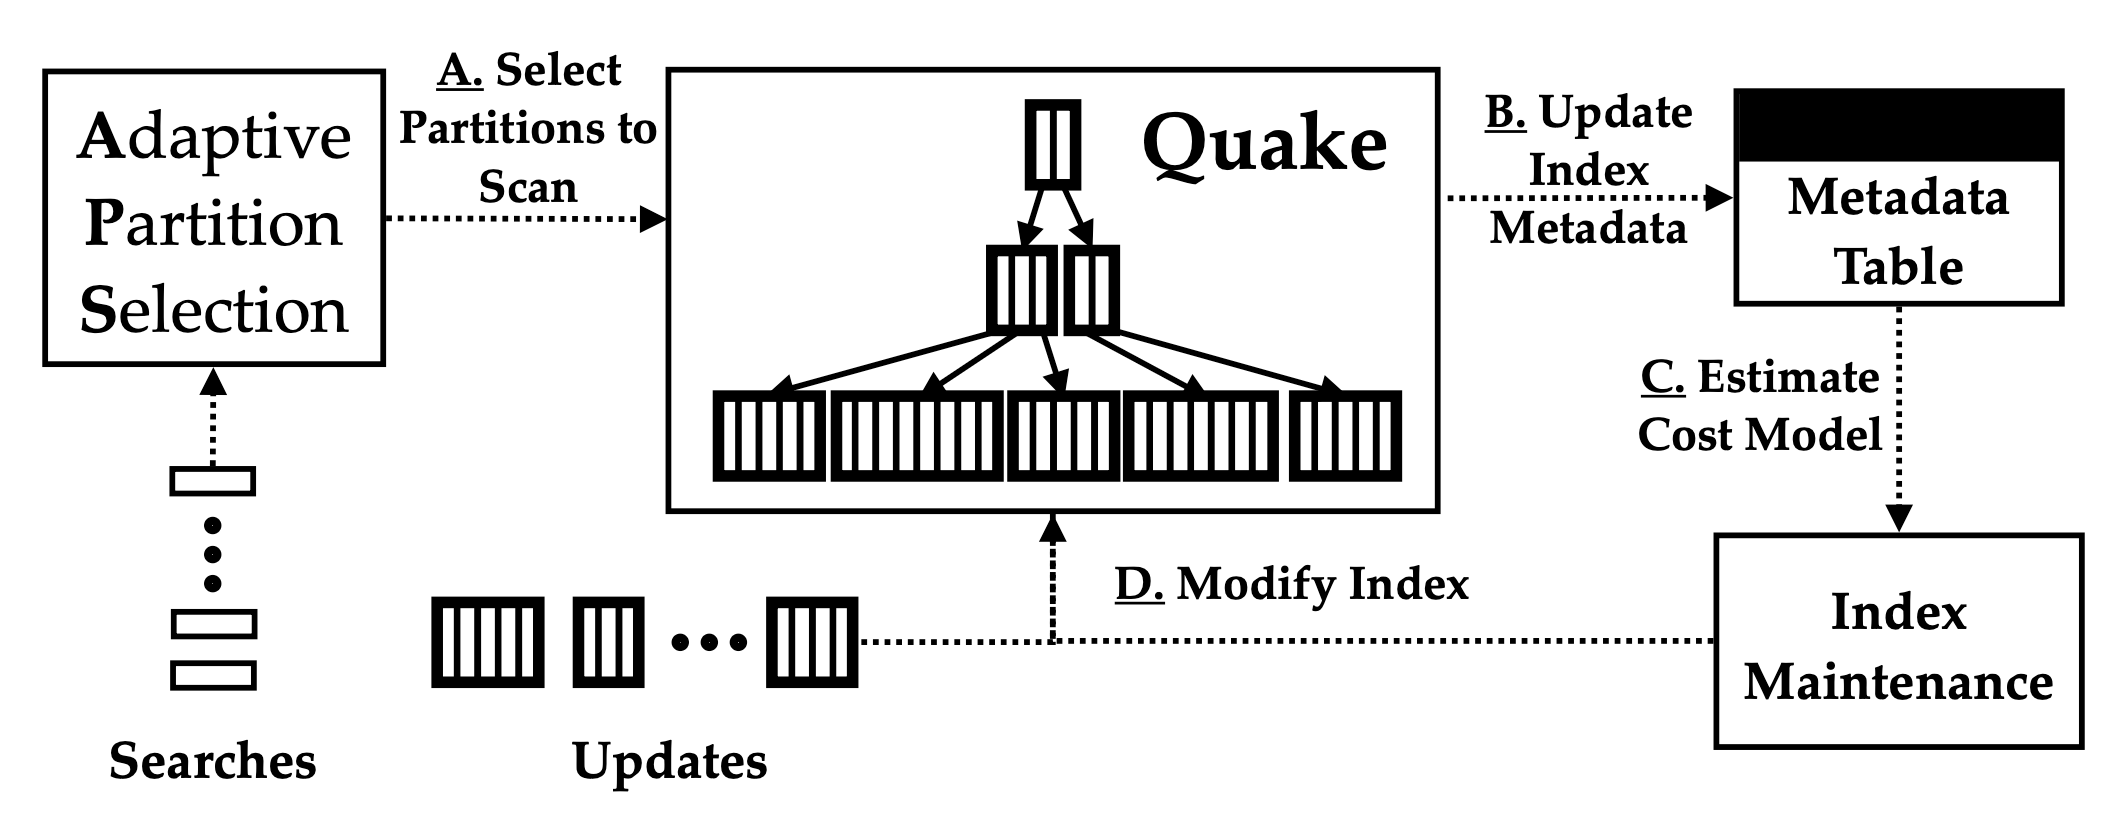
\includegraphics[width=9cm]{assets/quake_arch_2.png}
\end{center}

\blfootnote{Source at \href{https://github.com/marius-team/quake}{github.com/marius-team/quake}}
\end{frame}
\placelogotrue

%\placelogofalse
\begin{frame}{Quake Architecture}
\begin{center}
\centering
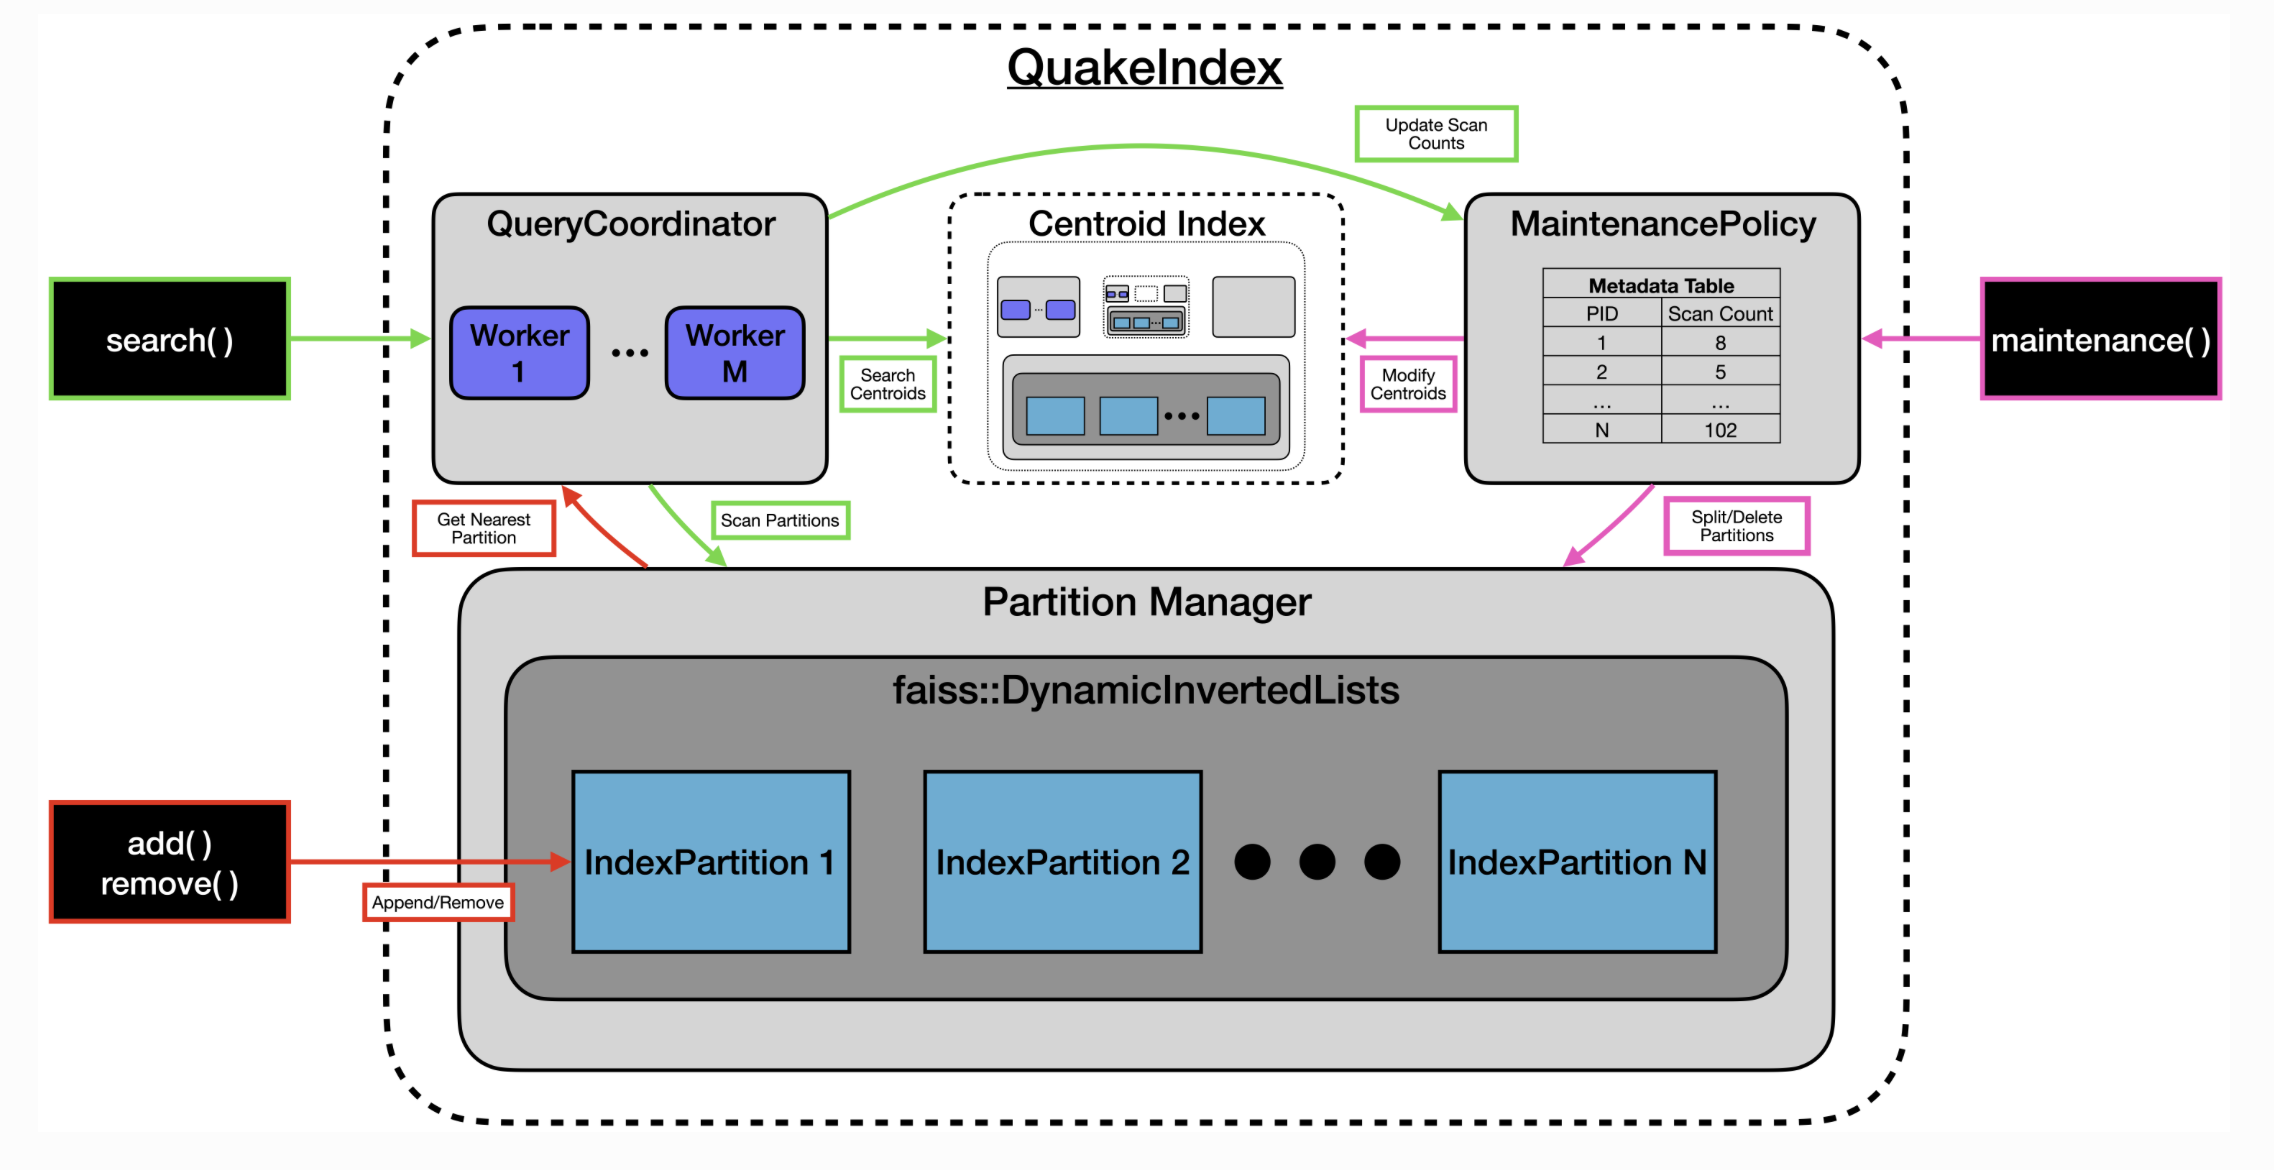
\includegraphics[width=12cm]{assets/quake_arch.png}

{\tiny From \href{https://marius-project.org/quake/architecture/architecture.html}{Quake Documentation}}
\end{center}
\end{frame}
%\placelogotrue
